
\de{ĐỀ THI HỌC KỲ I NĂM HỌC 2022-2023}{THPT Nguyễn Thị Định}
\begin{center}
	\textbf{PHẦN 1 - TRẮC NGHIỆM}
\end{center}
\Opensolutionfile{ans}[ans/0-TL-TN-NguyenThiDinh-HKII-NH22-23]
%Câu 1...........................
\begin{ex}%[0T9Y1-1]%[Dự án đề kiểm tra HKII NH22-23- Nguyễn Cường]%[THPT Nguyễn Thị Định]
Trong hệ tọa độ $Oxy$, cho $A(2;3)$, $B(10;13)$. Tìm tọa độ trung điểm $I$ của đoạn thẳng $AB$
	\choice
	{$(6;-8)$}
	{\True $(6;8)$}
	{$(12;16)$}
	{$(8;6)$}
	\loigiai{
		Tọa độ trung điểm $I$ của đoạn thẳng $AB$ là $\heva{&x=\dfrac{x_A+x_B}{2}\\&y=\dfrac{y_A+y_B}{2}}\Leftrightarrow\heva{&x=\dfrac{2+10}{2}=6\\&y=\dfrac{3+13}{2}=8.}$\\
		Suy ra tọa độ trung điểm của $AB$ là $I(6;8)$.
	}
\end{ex}
%Câu 2...........................
\begin{ex}%[0T7K2-1]%[Dự án đề kiểm tra HKII NH22-23- Nguyễn Cường]%[THPT Nguyễn Thị Định]
	Có bao nhiêu giá trị nguyên của tham số $m\in [-10;10]$ để với mọi $x\in\mathbb{R}$ biểu thức $f(x)=x^2+(m+2)x+8m+1$ luôn nhận giá trị dương?
	\choice
	{$11$}
	{\True $10$}
	{$27$}
	{Vô số}
	\loigiai{
		Ta có 
		\allowdisplaybreaks
		\begin{eqnarray*}
			x^2+(m+2)x+8m+1>0\,\forall x\in\mathbb{R}&\Leftrightarrow&\heva{&a>0\\&\Delta <0}\\
			&\Leftrightarrow&\heva{&1>0\\&(m+2)^2-4(8m+1)<0}\\
			&\Leftrightarrow&m^2-28m<0\\
			&\Leftrightarrow&0<m<28.
		\end{eqnarray*}
	Do $m$ nguyên và $m \in[-10;10]$ nên $m\in \{1;2;\cdots;9;10\}$.\\
	Vậy có $27$ giá trị nguyên của tham số $m$ thỏa mãn yêu cầu bài toán.
	}
\end{ex}
%Câu 3...........................
\begin{ex}%[0T8Y2-1]%[Dự án đề kiểm tra HKII NH22-23- Nguyễn Cường]%[THPT Nguyễn Thị Định]
	Có bao nhiêu cách xếp $4$ bạn học sinh thành một hàng dọc?
	\choice
	{$3!$}
	{$12$}
	{\True $4!$}
	{$\mathrm{A}_4^2$}
	\loigiai{
		Số cách xếp $4$ bạn học sinh thành một hàng dọc là $4!$.
	}
\end{ex}
%Câu 4...........................
\begin{ex}%[0T8B2-1]%[Dự án đề kiểm tra HKII NH22-23- Nguyễn Cường]%[THPT Nguyễn Thị Định]
	Có bao nhiêu cách $5$ sách Văn khác nhau và $7$ sách Toán khác nhau trên một kệ sách dài nếu $5$ sách Văn phải xếp kề nhau?
	\choice
	{\True $5!\cdot 8!$}
	{$2\cdot 5!\cdot 7!$}
	{$5!\cdot 7!$}
	{$12!$}
	\loigiai{
		Xếp $5$ sách Văn kề nhau có $5!$ cách.\\
		Ta xem $5$ sách Văn kề nhau là một bộ sách Văn.\\
		Khi đó, xếp số sách trên kệ là $8!$ cách.\\
		Vậy số cách xếp thỏa mãn yêu cầu bài toán là $5!\cdot 8!$ cách.
	}
\end{ex}
%Câu 5...........................
\begin{ex}%[0T3B2-3]%[Dự án đề kiểm tra HKII NH22-23- Nguyễn Cường]%[THPT Nguyễn Thị Định]
	\immini{Cho hàm số $f(x)=ax^2+bx+c$ với $a\ne 0$ có đồ thị như hình bên. Bảng xét dấu của hàm số $y=f(x)$ là
	\choice
	{\True 
%		\begin{center}
				
\begin{tikzpicture}
	\tkzTabInit[nocadre=false, lgt=1.2, espcl=2.5, deltacl=0.6]{$x$/0.6,$y$/0.6}
	{$-\infty$, $-1$,$1$, $+\infty$}
	\tkzTabLine {,-,0,+,0,-,}
\end{tikzpicture}
%	\end{center}
}
		{
%			\begin{center}
				
\begin{tikzpicture}
	\tkzTabInit[nocadre=false, lgt=1.2, espcl=2.5, deltacl=0.6]{$x$/0.6,$y$/0.6}
	{$-\infty$, $1$, $+\infty$}
	\tkzTabLine {,-,0,+,}
\end{tikzpicture}			
%	\end{center}
}
	{
%		\begin{center}
					
\begin{tikzpicture}
			\tkzTabInit[nocadre=false, lgt=1.2, espcl=2.5, deltacl=0.6]{$x$/0.6,$y$/0.6}
			{$-\infty$, $-1$, $+\infty$}
			\tkzTabLine {,+,0,-,}
		\end{tikzpicture}
%\end{center}
}
	{
%		\begin{center}
	
\begin{tikzpicture}
		\tkzTabInit[nocadre=false, lgt=1.2, espcl=2.5, deltacl=0.6]{$x$/0.6,$y$/0.6}
		{$-\infty$, $-1$,$1$, $+\infty$}
		\tkzTabLine {,+,0,-,0,+,}
	\end{tikzpicture}
%\end{center}
}
}
{
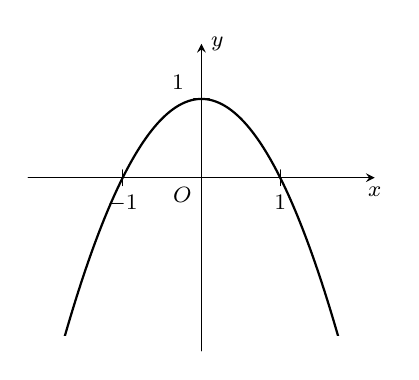
\begin{tikzpicture}[scale=1, line join=round, line cap=round, >=stealth,font=\footnotesize]
	\def\xmin{-2}\def\xmax{2}\def\ymin{-2}\def\ymax{1.5}
	\draw[->] (\xmin-0.2,0)--(\xmax+0.2,0) node[below]{$x$};
	\draw[->] (0,\ymin-0.2)--(0,\ymax+0.2) node[right]{$y$};
	\draw (0,0) node[below left]{$O$};
	\foreach \x in {-1,1}\draw (\x,0.1)--(\x,-0.1) node[below]{$\x$};
	\foreach \y in {1}\draw (0.1,\y)--(-0.1,\y) node[above left]{$\y$};
	\clip (\xmin,\ymin) rectangle (\xmax,\ymax);
	\draw[thick,smooth,samples=200,domain=\xmin:\xmax] plot (\x,{-1*((\x)^2)+0*\x+1});
\end{tikzpicture}
}
	\loigiai{
		Đồ thị hàm số cắt trục hoành tại $x=1$ và $x=-1$.\\
		Trên đoạn $[-1;1]$ đồ thị hàm số bên trên trục $Ox$ nên $y\ge 0$.\\
		Vậy bảng xét dấu của hàm số là 
		\begin{center}
			
\begin{tikzpicture}
				\tkzTabInit[nocadre=false, lgt=1.2, espcl=2.5, deltacl=0.6]{$x$/0.6,$y$/0.6}
				{$-\infty$, $-1$,$1$, $+\infty$}
				\tkzTabLine {,-,0,+,0,-,}
			\end{tikzpicture}
		\end{center}
	}
\end{ex}
%Câu 6...........................
\begin{ex}%[0T8K2-2]%[Dự án đề kiểm tra HKII NH22-23- Nguyễn Cường]%[THPT Nguyễn Thị Định]
	Một nhóm học sinh có $7$ em nam và $3$ em nữ. Hỏi có bao nhiêu cách xếp $10$ em này thành một hàng ngang sao cho hai vị trí đầu và cuối hàng là các em nam và không có $2$ em nữ nào ngồi cạnh nhau.
	\choice
	{\True $604\,800$}
	{$344\,000$}
	{$100\,800$}
	{$120\,120$}
	\loigiai{
	Xếp $7$ học sinh nam và nhất thiết nam đứng đầu hàng và cuối hàng có $7!$ cách.\\
	Khi đó, có $6$ vị trí xen giữa $7$ học sinh nam này.\\
	Ta chọn $3$ vị trí trong $6$ vị trí này để sắp xếp $3$ nữ vào nên có $\mathrm{A}_6^3$ cách.\\
	Vậy có $7!\cdot \mathrm{A}_6^3=604\,800$ cách.
	}
\end{ex}
%Câu 7...........................
\begin{ex}%[0T3Y2-2]%[Dự án đề kiểm tra HKII NH22-23- Nguyễn Cường]%[THPT Nguyễn Thị Định]
	Biểu thức nào sau đây là tam thức bậc hai?
	\choice
	{$f(x)=2x^3+3x+1$}
	{$f(x)=-5$}
	{$f(x)=x-4$}
	{\True $f(x)=-x^2+3x-5$}
	\loigiai{
		Tam thức bậc hai có dạng $f(x)=ax^2+bx+c$ với $a\ne 0$.\\
		Do đó, $f(x)=-x^2+3x-5$ là một tam thức bậc hai.
	}
\end{ex}
%Câu 8...........................
\begin{ex}%[0T8Y1-1]%[Dự án đề kiểm tra HKII NH22-23- Nguyễn Cường]%[THPT Nguyễn Thị Định]
	Có $3$ cuốn sách Toán khác nhau, $4$ cuốn sách Văn khác nhau và $7$ cuốn sách Anh Văn khác nhau. Một học sinh được chọn một quyển sách trong các quyển sách trên. Hỏi có bao nhiêu cách lựa chọn?
	\choice
	{$49$}
	{$84$}
	{$12$}
	{\True $14$}
	\loigiai{
		Số cách chọn $1$ quyển sách là $3+4+7=14$.
	}
\end{ex}
%Câu 9...........................
\begin{ex}%[0T8K2-2]%[Dự án đề kiểm tra HKII NH22-23- Nguyễn Cường]%[THPT Nguyễn Thị Định]
	Từ các chữ số $\{1;2;3;4;5;6\}$ lập được bao nhiêu số tự nhiên chẵn có bốn chữ số khác nhau mà luôn có mặt chữ số $1$?
	\choice
	{$144$}
	{\True $108$}
	{$24$}
	{$36$}
	\loigiai{
		Gọi $\overline{abcd}$ là số cần lập.\\
		Chọn vị trí cho chữ số $1$ có $3$ cách.\\
		Chọn chữ số $d$ có $3$ cách $d\in\{2;4;6\}$.\\
		Chọn $2$ chữ số trong $4$ chữ số và sắp xếp vào $2$ vị trí còn lại có $\mathrm{A}_4^2=12$.\\
		Vậy có $3\cdot 3\cdot 12=108$ số thỏa mãn.
	}
\end{ex}
%Câu 10...........................
\begin{ex}%[0T8Y3-1]%[Dự án đề kiểm tra HKII NH22-23- Nguyễn Cường]%[THPT Nguyễn Thị Định]
	Viết khai triển theo công thức nhị thức Newton của biểu thức $(x+y)^5$.
	\choice
	{$x^5+10x^4y+5x^3y^2+5x^2y^3+10xy^4+y^5$}
	{\True $x^5+5x^4y+10x^3y^2+10x^2y^3+5xy^4+y^5$}
	{$x^5-5x^4y+10x^3y^2-10x^2y^3+5xy^4-y^5$}
	{$x^5-5x^4y-10x^3y^2-10x^2y^3-5xy^4+y^5$}
	\loigiai{
		Ta có
		\allowdisplaybreaks
		\begin{eqnarray*}
			(x+y)^5&=&\mathrm{C}_5^0x^5+\mathrm{C}_5^1x^4y+\mathrm{C}_5^2x^3y^2+\mathrm{C}_5^3x^2y^3+\mathrm{C}_5^4xy^4+\mathrm{C}_5^5y^5\\
			&=&x^5+5x^4y+10x^3y^2+10x^2y^3+5xy^4+y^5.
		\end{eqnarray*}
	}
\end{ex}

%%=====Câu 11
\begin{ex}%[0T8Y1-2]%[Dự án đề kiểm tra HKII-22-23]%[Thầy Hóa]%[THPT Nguyễn Thị Định]
Bạn An có $4$ chiếc mũ khác nhau và $3$ áo khoác khác nhau để sử dụng khi đi học. Hỏi bạn An có bao nhiêu cách chọn $1$ chiếc mũ và $1$ áo khoác để sử dụng khi đi học?
\choice
{$3$}
{$7$}
{\True $12$}
{$1$}
\loigiai{
\begin{itemize}
	\item Chọn $1$ chiếc mũ trong $4$ chiếc mũ: có $4$ cách.
	\item Chọn $1$ áo khoác trong $3$ áo khoác: có $3$ cách.
\end{itemize}
Theo quy tắc nhân, có $4\cdot 3=12$ cách chọn.
}
\end{ex}

%%=====Câu 12
\begin{ex}%[0T7B2-1]%[Dự án đề kiểm tra HKII-22-23]%[Thầy Hóa]%[THPT Nguyễn Thị Định]
Tập nghiệm của bất phương trình $2x^2-5x+2\leq 0$ là
\choice
{$\left(\dfrac{1}{2};2\right)$}
{$\left(-\infty;\dfrac{1}{2}\right]\cup[2;+\infty)$}
{\True $\left[\dfrac{1}{2};2\right]$}
{$\left(-\infty; \dfrac{1}{2}\right) \cup(2;+\infty)$}
\loigiai{
Ta có $2x^2-5x+2=0\Leftrightarrow\hoac{&x=2\\&x=\dfrac{1}{2}.}$\\
Bảng xét dấu
\begin{center}

\begin{tikzpicture}
	\tkzTabInit[nocadre=false,lgt=3,espcl=3,deltacl=0.5]{$x$/1 ,$2x^2-5x+2$/1}
	{$-\infty$ , $\dfrac{1}{2}$ , $2$ , $+\infty$}
	\tkzTabLine{ , + , 0 , - , 0 , + , }
\end{tikzpicture}
\end{center}
Dựa vào bảng xét dấu, bất phương trình có nghiệm $x\in \left[\dfrac{1}{2};2\right]$.
}
\end{ex}

%%=====Câu 13
\begin{ex}%[0T8B3-2]%[Dự án đề kiểm tra HKII-22-23]%[Thầy Hóa]%[THPT Nguyễn Thị Định]
Xác định hệ số của $x^2$ trong khai triển biểu thức $(2x+1)^4$.
\choice
{$24x^2$}
{$6x^2$}
{$12$}
{\True $24$}
\loigiai{
Ta có $\begin{aligned}[t]
	(2x+1)^2&=\mathrm{C}_4^0(2x)^4+\mathrm{C}_4^1\cdot (2x)^3\cdot 1+\mathrm{C}_4^2\cdot (2x)^2\cdot 1^2+\mathrm{C}_4^3\cdot (2x)^1\cdot 1^3+\mathrm{C}_4^4\cdot 1^4\\
	&=16x^4+32x^3+24x^2+8x+1.
\end{aligned}$\\
Vậy hệ số của $x^2$ trong khai triển là $24$.
}
\end{ex}

%%=====Câu 14
\begin{ex}%[0T8B1-3]%[Dự án đề kiểm tra HKII-22-23]%[Thầy Hóa]%[THPT Nguyễn Thị Định]
Có $3$ bi xanh, $2$ bi đỏ và $4$ bi tím (các bi có kích thước khác nhau). Hỏi có bao nhiêu cách chọn ra $2$ bi có màu khác nhau?
\choice
{$36$}
{$9$}
{$24$}
{\True $26$}
\loigiai{
\begin{itemize}
	\item Chọn $1$ bi xanh và $1$ bi đỏ: có $3\cdot 2=6$ cách.
	\item Chọn $1$ bi xanh và $1$ bi tím: có $3\cdot 4=12$ cách.
	\item Chọn $1$ bi đỏ và $1$ bi tím: có $2\cdot 4=8$ cách.
\end{itemize}
Theo quy tắc cộng, có $6+12+8=26$ cách chọn ra $2$ bi có màu khác nhau.
}
\end{ex}

%%=====Câu 15
\begin{ex}%[0T9Y2-1]%[Dự án đề kiểm tra HKII-22-23]%[Thầy Hóa]%[THPT Nguyễn Thị Định]
Véc-tơ nào dưới đây là véc-tơ pháp tuyến của đường thẳng $2x+y-1=0$?
\choice
{\True $\vec{n}=(2;1)$}
{$\vec{n}=(1;2)$}
{$\vec{n}=(2;-1)$}
{$\vec{n}=(1;-1)$}
\loigiai{
Véc-tơ pháp tuyến của đường thẳng $2x+y-1=0$ là $\vec{n}=(2;1)$.
}
\end{ex}

%%=====Câu 16
\begin{ex}%[0T8Y2-1]%[Dự án đề kiểm tra HKII-22-23]%[Thầy Hóa]%[THPT Nguyễn Thị Định]
Số cách sắp xếp $6$ bạn học sinh nam và $4$ bạn học sinh nữ thành một hàng dọc là
\choice
{$6!\cdot 4!$}
{$\mathrm{C}_{10}^6\cdot \mathrm{C}_{10}^4$}
{\True $10!$}
{$6!+4!$}
\loigiai{
Mỗi cách sắp xếp $6$ bạn học sinh nam và $4$ bạn học sinh nữ thành một hàng dọc là một hoán vị của $10$ phần tử.\\
Vậy có $10!$ cách sắp xếp.
}
\end{ex}

%%=====Câu 17
\begin{ex}%[0T9K2-7]%[Dự án đề kiểm tra HKII-22-23]%[Thầy Hóa]%[THPT Nguyễn Thị Định]
Trong mặt phẳng tọa độ, một thiết bị âm thanh được phát từ vị trí $A(1;5)$. Người ta dự định đặt một máy thu tín hiệu trên đường thẳng có phương trình $x-2y-3=0$. Hỏi máy thu đặt ở vị trí nào dưới đây sẽ nhận được tín hiệu sớm nhất?
\choice
{$M(17;1)$}
{\True $M\left(\dfrac{17}{5};\dfrac{1}{5}\right)$}
{$M(12;1)$}
{$M\left(\dfrac{12}{5};\dfrac{1}{5}\right)$}
\loigiai{
Gọi $d$ là đường thẳng có phương trình $x-2y-3=0$.\\
Suy ra $d$ đi qua điểm $A(1;-1)$ và có véc-tơ pháp tuyến là $\vec{n}_d=(1;-2)$.\\
Suy ra véc-tơ chỉ phương của $d$ là $\vec{u}=(2;1)$.\\
Phương trình tham số của $d:\heva{&x=1+2t\\&y=-1+t.}$\\
Gọi $M$ là vị trí đặt máy thu tín hiệu. Để máy thu nhận được tín hiệu sớm nhất thì $M$ chính là hình chiếu của $A$ lên đường thẳng $d$. Suy ra $M\left(1+2t;-1+t\right)$ và $\vec{AM}=\left(2t;t-6\right)$ vuông góc với véc-tơ chỉ phương $\vec{u}=(2;1)$ của $d$. Do đó
\[2\cdot 2t+1\cdot (t-6)=0\Leftrightarrow 5t=6\Leftrightarrow t=\dfrac{6}{5}. \]
Suy ra $M\left(\dfrac{17}{5};\dfrac{1}{5}\right)$.
}
\end{ex}

%%=====Câu 18
\begin{ex}%[0T9B3-1]%[Dự án đề kiểm tra HKII-22-23]%[Thầy Hóa]%[THPT Nguyễn Thị Định]
Trong mặt phẳng $Oxy$, đường tròn $(C)\colon x^2+y^2-2x+6y+1=0$ có tâm $I$ và bán kính $R$ là
\choice
{\True $I(1;-3)$ và $R=3$}
{$I(1;-3)$ và $R=\sqrt{10}$}
{$I(-1;3)$ và $R=3$}
{$I(2;-6)$ và $R=\sqrt{39}$}
\loigiai{
Ta có $\heva{&-2a=-2\\&-2b=6\\&c=1}\Leftrightarrow \heva{&a=1\\&b=-3\\&c=1.}$\\
Suy ra $(C)$ có tâm $I(1;-3)$ và $R=\sqrt{a^2+b^2-c}=\sqrt{1+9-1}=3$.
}
\end{ex}

%%=====Câu 19
\begin{ex}%[0T8B2-1]%[Dự án đề kiểm tra HKII-22-23]%[Thầy Hóa]%[THPT Nguyễn Thị Định]
Một lớp có $45$ học sinh. Hỏi có bao nhiêu cách chọn $3$ học sinh để làm vệ sinh lớp học trong một ngày?
\choice
{$90$}
{$24\,360$}
{\True $14\,190$}
{$900$}
\loigiai{
Mỗi cách chọn $3$ học sinh trong $45$ học sinh để làm vệ sinh lớp học trong một ngày là một tổ hợp chập $3$ của $45$ phần tử.\\
Vậy có $\mathrm{C}_{45}^3=14\,190$ cách chọn.
}
\end{ex}

%%=====Câu 20
\begin{ex}%[0T9B3-2]%[Dự án đề kiểm tra HKII-22-23]%[Thầy Hóa]%[THPT Nguyễn Thị Định]
Phương trình nào là phương trình của đường tròn tâm $I(-3;4)$, có bán kính $R=2$?
\choice
{$(x-3)^2+(y-4)^2=4$}
{$(x+3)^2+(y-4)^2=2$}
{$(x+3)^2+(y+4)^2=4$}
{\True $(x+3)^2+(y-4)^2=4$}
\loigiai{
Phương trình đường tròn tâm $I(-3;4)$, có bán kính $R=2$ là
\[(x+3)^2+(y-4)^2=4. \]
}
\end{ex}



\Closesolutionfile{ans}


\begin{center}
	\textbf{PHẦN 2 - TỰ LUẬN}
\end{center}



	\begin{bt}%[0T7B2-1]%[Dự án đề kiểm tra HKII-NH22-23, Dương Phước Sang]%[THPT Nguyễn Thị Định-TP.HCM]
		Giải bất phương trình $-2x^2-5x-3 \geq 0$.
		\loigiai{
			Cho $-2x^2-5x-3= 0 \Leftrightarrow \hoac{&x=-1\\&x=-\dfrac{3}{2}.}$\\
			Bảng xét dấu
			\begin{center}
				
\begin{tikzpicture}
					\tkzTabInit[nocadre=true,lgt=2.8,espcl=2]
					{$x$/1,$-2x^2-5x-3$/1}
					{$-\infty$,$-\dfrac{3}{2}$,$-1$,$+\infty$}
					\tkzTabLine{,-,$0$,+,$0$,-,}
				\end{tikzpicture}
			\end{center}
			Vậy tập nghiệm của bất phương trình $-2x^2-5x-3 \geq 0$ là $S=\left[-\dfrac{3}{2};-1\right]$.
		}
	\end{bt}
	
	\begin{bt}%[0T8B3-1]%[Dự án đề kiểm tra HKII-NH22-23, Dương Phước Sang]%[THPT Nguyễn Thị Định-TP.HCM]
		Khai triển theo công thức nhị thức Newton $(2x+3)^4$.
		\loigiai{
			Ta có 
			\allowdisplaybreaks
			$\begin{aligned}[t]
				(2x+3)^4
				&=\mathrm{C}_4^0 \,(2x)^4+\mathrm{C}_4^1 \,(2x)^3\cdot 3+\mathrm{C}_4^2 \,(2x)^2\cdot 3^2+\mathrm{C}_4^3 \,(2x)\cdot 3^3+\mathrm{C}_4^4 3^4\\
				&=16x^4+96x^3+216x^2+216x+81.
			\end{aligned}$
		}
	\end{bt}
	
	\begin{bt}%[0T8B1-2]%[Dự án đề kiểm tra HKII-NH22-23, Dương Phước Sang]%[THPT Nguyễn Thị Định-TP.HCM]
		\immini{
			Một ổ khóa có $3$ vòng số (mỗi vòng gồm $10$ số, từ $0$ đến $9$) như hình. Người dùng cần đặt mật mã cho khóa là một dãy số có $3$ chữ số. Để mở khóa, cần xoay các vòng số để dãy số phía trước khóa trùng với mật mã đã chọn. Có bao nhiêu cách chọn mật mã cho khóa?}
		{\vspace{-0.5cm}
			\definecolor{dodgerblue}{rgb}{0.12, 0.56, 1.0}
			\definecolor{gainsboro}{rgb}{0.86, 0.86, 0.86}
			\definecolor{outerspace}{rgb}{0.25, 0.29, 0.3}
			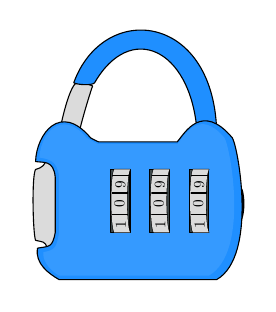
\begin{tikzpicture}[line join=round, line cap=round,scale=.5,transform shape]
				\clip (-2.8,-3.3) rectangle (2.8,3.2);
				\tikzset{so/.pic={
						\def\s{ 
							(-1,-.8)
							..controls +(30:.2) and +(150:.2) .. (.6,-.8)--
							(.6,-.4)
							..controls +(150:.2) and +(30:.2) .. (-1,-.4);
						}
						\draw[fill=outerspace] (-1,-.8) rectangle (.6,-.3);
						
						\draw \s;
						\fill[gainsboro] \s;
						\draw (.45,-.36)--(.45,-.77) (0,-.35)--(0,-.74) (-.55,-.35)--(-.55,-.74);
						\node[scale=1.1,inner sep=0,align=left,
						font=\fontfamily{qag}\selectfont] at (-.8,-.57) 
						{1};
						\node[scale=1.1,inner sep=0,align=left,
						font=\fontfamily{qag}\selectfont] at (-.26,-.53) 
						{0};
						\node[scale=1.1,inner sep=0,align=left,
						font=\fontfamily{qag}\selectfont] at (.22,-.56) 
						{9};
						%\fill[dodgerblue] \s;
				}}
				
				\tikzset{khoa/.pic={
						%xám
						\draw[fill=outerspace] (2.64,-.9)
						..controls +(-70:.2) and +(70:.2) .. (2.64,-1.65)
						..controls +(80:.15) and +(-80:.15) .. cycle
						;
						\def\x{ 
							(-2.3,-.1)
							..controls +(-110:.2) and +(15:.2) ..(-2.6,-.4)
							..controls +(-120:.2) and +(110:.2) ..(-2.6,-2.2)
							..controls +(-15:.2) and +(110:.2) ..(-2.3,-2.4)--(-2,-2.4)--(-2,-.1)--cycle
							
							(-2,.5)
							..controls +(80:.2) and +(-130:.3) ..(-1.6,1.77)
							..controls +(20:.2) and +(160:.2) ..(-1.15,1.72)
							..controls +(-110:.3) and +(80:.2) ..(-1.5,.5)--cycle
							
							;}
						
						\fill[gainsboro] \x;
						\draw \x;
						
						\def\k2{ 
							(-1.63,1.8)
							..controls +(-30:.1) and +(-130:.1) ..(-1.1,1.8)
							..controls +(60:1.8) and +(95:2.1) ..(1.5,.6)--(2,.6)
							..controls +(92:3) and +(70:2.2) ..cycle
							;}
						
						\fill[dodgerblue] \k2;
						\draw \k2;
						
						\def\K{ 
							(1,.3)--(-1,.3)
							..controls +(170:.02) and +(-30:.02) .. (-1.2,.4)
							..controls +(130:1.2) and +(88:.7) ..  (-2.6,-.2)
							..controls +(-10:.2) and +(95:.45) ..(-2.1,-.6)--(-2.1,-2)
							..controls +(-100:.4) and +(10:.3) ..  (-2.55,-2.4)
							..controls +(-100:.4) and +(150:.3) ..  (-2,-3.2)--(2,-3.2)
							..controls +(30:1.2) and +(-60:.3) ..  (2.4,.4)
							..controls +(130:1.2) and +(50:.3) ..  cycle
							;}
						\def\k1{ 
							(1,.24)--(-1,.24)
							..controls +(170:.02) and +(-30:.02) .. (-1.3,.4)
							..controls +(130:1) and +(88:.6) ..  (-2.5,-.1)
							..controls +(-10:.2) and +(95:.45) ..(-2,-.6)--(-2,-2)
							..controls +(-100:.4) and +(10:.3) ..  (-2.4,-2.5)
							..controls +(-100:.2) and +(150:.3) ..  (-2,-3.1)--(1.8,-3.1)
							..controls +(30:1.2) and +(-60:.3) ..  (2.2,.4)
							..controls +(130:1) and +(50:.3) ..  cycle
							;}
						\fill[dodgerblue] \K;
						\draw \K;
						\fill[dodgerblue!90] \k1;
						
				}}
				\path
				(0,0)pic[scale=1]{khoa}
				(-1,-1)pic[rotate=90,scale=1]{so}
				(0,-1)pic[rotate=90,scale=1]{so}
				(1,-1)pic[rotate=90,scale=1]{so}
				;			
		\end{tikzpicture}}
		\loigiai{
			Mật mã của khóa có dạng $\overline{abc}$ với $a,b,c \in \big\{0;1;2;\ldots;9\big\}$.\\
			Số cách chọn cho mỗi vị trí số $a$, $b$, $c$ là $10$.\\
			Để có một mật khẩu cần thực hiện đủ $3$ bước chọn từng vị trí trong chuỗi, do đó có 
			$$10\cdot 10\cdot 10=1000 \text{  mật mã cho khóa}.$$
		}
	\end{bt}
	
	\begin{bt}%[0T9B2-2]%[Dự án đề kiểm tra HKII-NH22-23, Dương Phước Sang]%[THPT Nguyễn Thị Định-TP.HCM]
		Cho $3$ điểm $A(5;-2)$, $B(-1;1)$ và $C(0;3)$. Hãy viết phương trình tổng quát của đường cao $AH$ của tam giác $ABC$.
		\loigiai{
			Đường cao $AH$ của $\triangle ABC$ đi qua $A(5;-2)$ và nhận $\vec{BC}=(1;2)$ làm véc-tơ pháp tuyến.\\
			Do đó $AH$ có phương trình tổng quát là $1(x-5)+2(y+2)=0 \Leftrightarrow x+2y-1=0$.
		}
	\end{bt}
	
	\begin{bt}%[0T9K3-2]%[Dự án đề kiểm tra HKII-NH22-23, Dương Phước Sang]%[THPT Nguyễn Thị Định-TP.HCM]
		Viết phương trình đường tròn đi qua $3$ điểm $M(2;-2)$, $N(4;-1)$ và $P(-1;5)$.
		\loigiai{
			Xét $(C)\colon x^2+y^2-2ax-2by+c=0$ là đường tròn đi qua $M(2;-2)$, $N(4;-1)$ và $P(-1;5)$.\\
			Khi đó ta có hệ phương trình 
			$\heva{&4-4a+4b+c=0\\&17-8a+2b+c=0\\&26+2a-10b+c=0}
			\Leftrightarrow \heva{&a=\dfrac{45}{34}\\&b=\dfrac{63}{34}\\&c=-\dfrac{172}{17}.}$\\
			Vậy $(C)\colon x^2+y^2-\dfrac{45}{17}x-\dfrac{63}{17}y-\dfrac{172}{17}=0$  là đường tròn đi qua $M(2;-2)$, $N(4;-1)$ và $P(-1;5)$.
		}
	\end{bt}
	
	\begin{bt}%[0T9B4-1]%[Dự án đề kiểm tra HKII-NH22-23, Dương Phước Sang]%[THPT Nguyễn Thị Định-TP.HCM]
		Cho $(E)\colon \dfrac{x^2}{100}+\dfrac{y^2}{36}=1$. Hãy xác định độ dài trục lớn, độ dài trục nhỏ, tiêu cự và tọa độ hai tiêu điểm của $(E)$.
		\loigiai{
			Với $\heva{&a^2=100\\&b^2=36}$ ta có $\heva{&a=10\\&b=6}$ và $c=\sqrt{a^2-b^2}=8$.\\
			Từ đó $(E)$ có độ dài trục lớn là $2a=20$.\\
			\phantom{Từ đó} $(E)$ có độ dài trục nhỏ là $2b=12$.\\
			\phantom{Từ đó} $(E)$ có tiêu cự là $2c=16$.\\
			\phantom{Từ đó} Và $2$ tiêu điểm của $(E)$ là $F_1(-8;0)$, $F_2(8;0)$.
		}
	\end{bt}